\subsection{Theoretische Grundlagen}

Die Funktionsweise  der meisten Digitalkameras kann anhand eines Linsensystems
erkl\"art werden, der ein Gegenstand auf ein CCD (engl. \textit{Charge Coupled
Device})  auch  \textit{Bildsensor}  gennant,  projeziert   (siehe   Abbildung
\ref{fig:linseccd}).

\begin{figure}[h!]
    \centering
    \begin{subfigure}[b]{.45\linewidth}
        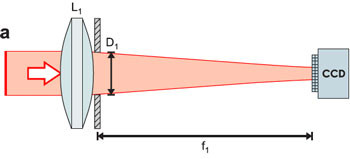
\includegraphics[width=\textwidth]{imLinseCCD}
        \caption{Linse, die ein Gegenstand auf den Kamerasensor abbildet \cite{ref:perfektfokusiert}}
        \label{fig:linseccd}
    \end{subfigure}
    \begin{subfigure}[b]{.45\linewidth}
        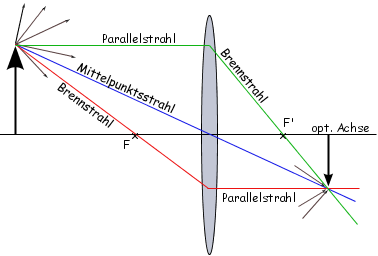
\includegraphics[width=\textwidth]{imLinsengleichung}
        \caption{Eine Visualisierung der Linsengleichung \cite{ref:Linsengleichung}}
        \label{fig:linsengleichung}
    \end{subfigure}
\end{figure}

Sind die physikalischen Dimensionen  dieses Sensors bekannt, so kann mit Hilfe
der Linsengleichung  (siehe  Abbildung \ref{fig:linsengleichung} und Gleichung
\ref{eq:linsengleichung}) das Linsensystem berechnet werden und somit von  der
Bildgr\"osse    auf    der    realen    Gegenstandsgr\"osse   eines   Objektes
zur\"uckgeschlossen werden. Die Linsengleichung lautet:

\begin{equation}
    \frac{1}{f} = \frac{1}{g} + \frac{1}{b}
    \label{eq:linsengleichung}
\end{equation}

Weiter kann der Vergr\"osserungsfaktor $\beta$ berechnet werden:

\begin{equation}
    \beta = \frac{B}{G} = \frac{b}{g}
\end{equation}


\subsection{Versuchsaufbau}

Nenndaten der Kamera:
    
\begin{itemize}
    \item Aufl\"osung Sensor : 1024x768 Pixel
    \item Gegenstandsweite : \SI{13}{\centi\meter}
    \item Cell Size : \SI{4.65 x 4.65}{\micro\meter}
    \item Brennweite : \SI {6}{\milli\meter}
\end{itemize}

Der  Studentenausweis  wird  direkt  von  Oben  fotografiert  und die  Distanz
zwischen   der   Linse    und    des    Studentenausweises    wird    gemessen
(\SI{13}{\centi\meter}).


\subsection{Ergebnisse}

\begin{figure}[h!]
    \centering
    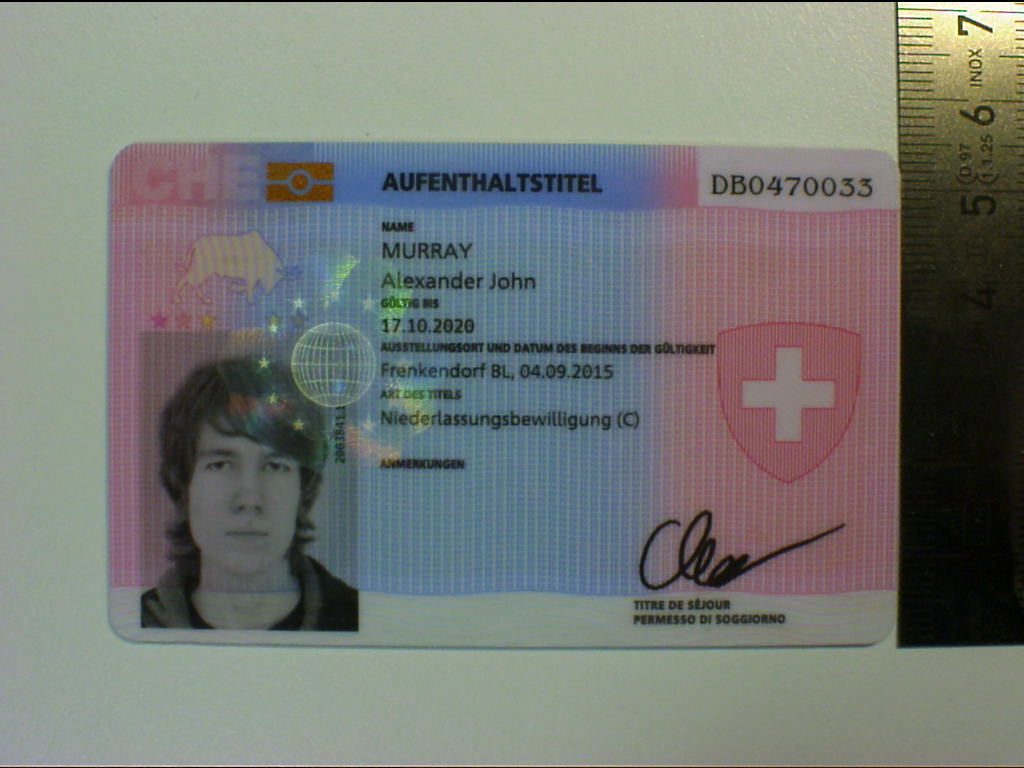
\includegraphics[width=.6\linewidth]{Posten_2_fuckface.png}
    \caption{Aufgenommenes Bild des Studentenausweises}
\end{figure}

Die Dimensionen  in  Pixel des Aufgenommenn Studentenausweises wurde mit einem
Bildverarbeitungsprogramm ermittelt. Sie ergibt sich als 787 x  511  Pixel. Da
die  Sensoraufl\"osung bekannt ist (1024 x 786 Pixel) sowie auch die Cell Size
(\SI{4.65  x  4.65}{\micro\meter})  kann  die Abbildungsgr\"osse des Ausweises
berechnet werden.

\begin{align*}
    B_x = 787\cdot\SI{4.65}{\micro\meter} &= \SI{3659.55}{\micro\meter} \\
    B_y = 511\cdot\SI{4.65}{\micro\meter} &= \SI{2376.15}{\micro\meter}
\end{align*}

Der  Abstand  zum  Brennpunkt  $f$  ist  in   den  Nenndaten  der  Kamera  als
\SI{6}{\milli\meter} angegeben. Der Abstand zum Gegenstand $g$ wurde gemessen.
So    kann    die    Abbildungsabstand    $b$    mit    der    Linsengleichung
(\ref{eq:linsengleichung}) berechnet werden.

\begin{equation*}
    b = \frac{1}{\frac{1}{f}-\frac{1}{g}} = \SI{6.29}{\milli\meter}
\end{equation*}

Mit $g$ und $b$ kann der Vergr\"osserungsfaktor $\beta$ berechnet werden:

\begin{equation*}
    \beta = \frac{b}{g} = 0.04838
\end{equation*}

Und folglich kann somit die Gegenstandsgr\"osse berechnet werden:

\begin{align*}
    G_x = \frac{B_x}{\beta} &= \SI{75.63}{\milli\meter} \\
    G_y = \frac{B_y}{\beta} &= \SI{49.11}{\milli\meter}
\end{align*}


\subsection{Erkenntnisse}

Die  berechnete Gegenstandsgr\"osse (\SI{49.11}{\milli\meter}) ist  ein  wenig
kleiner   als   die   gemessene  Gegenstandsgr\"osse  (\SI{54}{\milli\meter}).

Die  Ursache hierf\"ur kann  einerseits  auf  Ungenauigkeiten  der  gemessenen
Distanz $g$  zwischen  Gegenstand  und Linse zur\"uckgef\"uhrt werden (weil es
nicht ganz klar war wo die Linse im Objektiv anf\"angt), anderseits  kann  der
Fehler auch davon stammen, dass das Objektiv nicht nur aus einer Linse besteht
sondern aus einem Linsensystem.

